%%%%%%%%%%%%%%%%%%%%%%%%%%%%%%%%%%%%%%%%%
% Beamer Presentation
% LaTeX Template
% Version 1.0 (10/11/12)
%
% This template has been downloaded from:
% http://www.LaTeXTemplates.com
%
% License:
% CC BY-NC-SA 3.0 (http://creativecommons.org/licenses/by-nc-sa/3.0/)
%
%%%%%%%%%%%%%%%%%%%%%%%%%%%%%%%%%%%%%%%%%

%----------------------------------------------------------------------------------------
%	PACKAGES AND THEMES
%----------------------------------------------------------------------------------------

\documentclass{beamer}

\mode<presentation> {

% The Beamer class comes with a number of default slide themes
% which change the colors and layouts of slides. Below this is a list
% of all the themes, uncomment each in turn to see what they look like.

%\usetheme{default}
%\usetheme{AnnArbor}
%\usetheme{Antibes}
%\usetheme{Bergen}
%\usetheme{Berkeley}
%\usetheme{Berlin}
%\usetheme{Boadilla}
%\usetheme{CambridgeUS}
%\usetheme{Copenhagen}
\usetheme{Darmstadt}
%\usetheme{Dresden}
%\usetheme{Frankfurt}
%\usetheme{Goettingen}
%\usetheme{Hannover}
%\usetheme{Ilmenau}
%\usetheme{JuanLesPins}
%\usetheme{Luebeck}
%\usetheme{Madrid}
%*\usetheme{Malmoe}
%\usetheme{Marburg}
%\usetheme{Montpellier}
%\usetheme{PaloAlto}
%\usetheme{Pittsburgh}
%\usetheme{Rochester}
%\usetheme{Singapore}
%\usetheme{Szeged}
%\usetheme{Warsaw}

% As well as themes, the Beamer class has a number of color themes
% for any slide theme. Uncomment each of these in turn to see how it
% changes the colors of your current slide theme.

%\usecolortheme{albatross}
%\usecolortheme{beaver}
%\usecolortheme{beetle}
%\usecolortheme{crane}
%\usecolortheme{dolphin}
%\usecolortheme{dove}
%\usecolortheme{fly}
%\usecolortheme{lily}
\usecolortheme{orchid}
%\usecolortheme{rose}
%\usecolortheme{seagull}
%\usecolortheme{seahorse}
%\usecolortheme{whale}
%\usecolortheme{wolverine}

%\setbeamertemplate{footline} % To remove the footer line in all slides uncomment this line
%\setbeamertemplate{footline}[page number] % To replace the footer line in all slides with a simple slide count uncomment this line

%\setbeamertemplate{navigation symbols}{} % To remove the navigation symbols from the bottom of all slides uncomment this line
}


\usepackage{graphicx} % Allows including images
\usepackage{booktabs} % Allows the use of \toprule, \midrule and \bottomrule in tables
\usepackage{xspace}
\usepackage{caption}
\usepackage{subfigure}
\usepackage[english,brazil]{babel}
\usepackage[utf8]{inputenc}

%Renomeia o nome padrao das figuras.
\renewcommand{\figurename}{Figura}
\renewcommand{\tablename}{Tabela}
%----------------------------------------------------------------------------------------
%	TITLE PAGE
%----------------------------------------------------------------------------------------

\title[Computação Gráfica]{Modelo de Iluminação} % The short title appears at the bottom of every slide, the full title is only on the title page

\author{Uéliton Freitas} % Your name
\institute[UFMS] % Your institution as it will appear on the bottom of every slide, may be shorthand to save space
{
Universidade Católica Don Bosco - UCDB \\ % Your institution for the title page
\medskip
\textit{freitas.ueliton@gmail.com} % Your email address
}
\date{\today} % Date, can be changed to a custom date


\begin{document}

\begin{frame}
\titlepage % Print the title page as the first slide
\end{frame}

\begin{frame}
\frametitle{Sumário} % Table of contents slide, comment this block out to remove it
\tableofcontents % Throughout your presentation, if you choose to use \section{} and \subsection{} commands, these will automatically be printed on this slide as an overview of your presentation
\end{frame}




%----------------------------------------------------------------------------------------
%	PRESENTATION SLIDES
%----------------------------------------------------------------------------------------

%------------------------------------------------
\section{Introdução} 
%------------------------------------------------

%\section{Speeded-Up Robust Features - SURF} % A subsection can be created just before a set of slides with a common theme to further break down your presentation into chunks
%\section{Baf Of Features and Colors}

%\section{Refer\^encias}
%%%%%%%%%%%%%%%%%%%%%%%%%%%%%%%%%%%%%%%%%%%%%%%%%%%%%%%%%%%%%%%%%%%%%%%%%%%%%%%%%%%%%%%%%%
\begin{frame}
\frametitle{Introdução}

		\begin{block}{Introdução}
		\begin{itemize}
			\item Os modelos físicos envolvem vários fatores como \textbf{propriedade dos materiais},\textbf{posições} dos objetos em relação a luz e outros objetos, além das características das fontes de luz.
			\begin{itemize}
				\item Os objetos podem ser transparentes ou opacos, podem ser finos ou  mais grosseiros.
				\item Fontes de luz podem ter vários formatos, cores e posições.
			\end{itemize}
			\item Os \textbf{Modelos de Iluminação} em computação gráfica são, na maioria das vezes, \textbf{aproximações} das leis da física que descrevem efeitos de luz sobre as superfícies.			 
		\end{itemize}
	\end{block}
	
\end{frame}



%%%%%%%%%%%%%%%%%%%%%%%%%%%%%%%%%%%%%%%%%%%%%%%%%%%%%%%%%%%%%%%%%%%%%%%%%%%%%%%%%%%%%%%%%%
\section{Fontes de Luz}
\begin{frame}
\frametitle{Fontes de Luz}

	\begin{block}{Fontes de Luz}
		\begin{itemize}
			\item Qualquer objeto brilhante é uma \textbf{fonte de luz} e emite luz e contribui para os efeitos de luz dos outros objetos da cena.
			\item \textbf{Fontes de Luz} podem ter diferentes formas e características (posição, cor, direção de emissão) podendo emitir ou refletir luz.
			\item Em aplicações gráficas de \textbf{tempo real}, muitas vezes são utilizados modelos simples de iluminação para obter um melhor \textbf{custo computacional}.
		\end{itemize}
	\end{block}
\end{frame}

%%%%%%%%%%%%%%%%%%%%%%%%%%%%%%%%%%%%%%%%%%%%%%%%%%%%%%%%%%%%%%%%%%%%%%%%%%%%%%%%%%%%%%%%%%
\begin{frame}
\frametitle{Fontes de Luz}

	\begin{block}{Fonte de Luz Puntual}
		\begin{itemize}
			\item É o modelo de luz mais simples.
			\begin{itemize}
				\item Possui uma posição.
				\item Defini-se a cor que será emitida.
				\item Os raios de luz são gerados em \textbf{direções radiais divergentes} a partir do ponto da luz.
			\end{itemize}
		\end{itemize}
	\end{block}
		\begin{figure}[!h]
			\begin{center}
			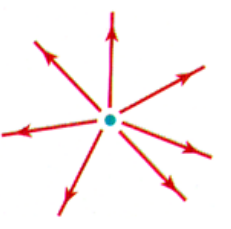
\includegraphics[width=0.2\textwidth]{Figures/FonPun}
			\end{center}
		\end{figure}
\end{frame}

%%%%%%%%%%%%%%%%%%%%%%%%%%%%%%%%%%%%%%%%%%%%%%%%%%%%%%%%%%%%%%%%%%%%%%%%%%%%%%%%%%%%%%%%%%
\begin{frame}
\frametitle{Fontes de Luz}

	\begin{block}{Fonte de Luz Infinitamente Distantes}
		\begin{itemize}
			\item Uma fonte de luz grande(p.ex Sol) que está bem longe da cena pode ser aproximado com um ponto emissor bem distante dos objetos.
			\begin{itemize}
				\item A iluminação é provida em uma única direção.
			\end{itemize}
			\item Uma fonte de luz distante é simulada definindo uma \textbf{cor} e uma \textbf{direção} de emissão de raios. Não é necessário definir uma posição.
		\end{itemize}
	\end{block}
		\begin{figure}[!h]
			\begin{center}
			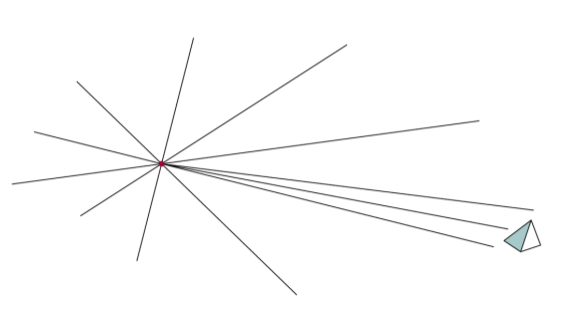
\includegraphics[width=0.6\textwidth]{Figures/FonDis}
			\end{center}
	\end{figure}
\end{frame}

%%%%%%%%%%%%%%%%%%%%%%%%%%%%%%%%%%%%%%%%%%%%%%%%%%%%%%%%%%%%%%%%%%%%%%%%%%%%%%%%%%%%%%%%%%
\begin{frame}
\frametitle{Fontes de Luz}

	\begin{block}{Atenuação Radial da Intensidade}
		\begin{itemize}
			\item A energia de radiação de uma fonte de luz em uma distância $d_l$ da origem, tem sua \textbf{amplitude} atenuada  por um fator $\frac{1}{d^{2}_{l}}$.
			\begin{itemize}
				\item Uma superfície próxima a fonte de luz recebe maior intensidade de luz.
				\item Para uma \textbf{iluminação realística} esta atenuação deve ser considerada.
			\end{itemize}
			\item Na prática uma atenuação $\frac{1}{d^{2}_{l}}$ para fontes de luz puntuais não produz efeitos realísticos.
			\begin{itemize}
				\item Há uma alta variação de intensidade em objetos próximos a fonte de luz e uma baixa variação para objetos que estão longe da fonte.
			\end{itemize}
		\end{itemize}
	\end{block}
\end{frame}

%%%%%%%%%%%%%%%%%%%%%%%%%%%%%%%%%%%%%%%%%%%%%%%%%%%%%%%%%%%%%%%%%%%%%%%%%%%%%%%%%%%%%%%%%%
\begin{frame}
\frametitle{Fontes de Luz}

	\begin{block}{Atenuação Radial da Intensidade}
		\begin{itemize}
			\item Para produzir efeitos mais realísticos com fonte de luz puntuais usamos:
				\begin{equation*}
					f(d_l) = \frac{1}{a_0 + a_1d_l + a_2d^{2}_{l}}
				\end{equation*}
			\item Os valores de $a_0,a_1$ e $a_2$ podem ser ajustados para produzir efeitos de atenuações desejados.
			\begin{itemize}
				\item Valores grandes podem ser assinalados para $a_0$ quando $d_l$ é muito pequeno para prevenir que $f(d_l)$ de ficar muito grande.
			\end{itemize}
		\end{itemize}
	\end{block}
\end{frame}

%%%%%%%%%%%%%%%%%%%%%%%%%%%%%%%%%%%%%%%%%%%%%%%%%%%%%%%%%%%%%%%%%%%%%%%%%%%%%%%%%%%%%%%%%%
\begin{frame}
\frametitle{Fontes de Luz}

	\begin{block}{Atenuação Radial da Intensidade}
		\begin{itemize}
			\item Este cálculo não pode ser aplicado para fontes de luz no ``infinito'' porque a distância $d_l$ é indeterminada.
			\item Um outro problema que é que quase todos os pontos estarão a mesma distância da fonte de luz. (baixo realismo).
			\item Para resolver o problema:
			$ f(d_l) = \left\{ 
  					\begin{array}{l l}
   						 1 & \quad \text{se a fonte de luz está no infinito}\\
    						\frac{1}{a_0 + a_1d_l + a_2d^{2}_{l}} & \quad \text{se a fonte de luz é local}
  					\end{array} \right.$ 
		\end{itemize}
	\end{block}
\end{frame}


%%%%%%%%%%%%%%%%%%%%%%%%%%%%%%%%%%%%%%%%%%%%%%%%%%%%%%%%%%%%%%%%%%%%%%%%%%%%%%%%%%%%%%%%%%
\section{Fontes de Luz Direcional e Efeito de Holofote}
\begin{frame}
\frametitle{Fontes de Luz}

	\begin{block}{Efeito de Holofote}
		\begin{itemize}
			\item Uma fonte e luz pontual pode ser direcionada para produzir um efeito de \textbf{luz direcional} ou holofote.
			\begin{itemize}
				\item Se o objeto está fora dos limites direcionais ele é eliminado da iluminação.
			\end{itemize}
			\item Uma \textbf{fonte de luz direcional} pode ser definida por uma \textbf{posição}, um \textbf{vetor direcional} e um limite angular $\theta$ a partir deste vetor.				 
		\end{itemize}
	\end{block}

	\begin{figure}[!h]
			\begin{center}
			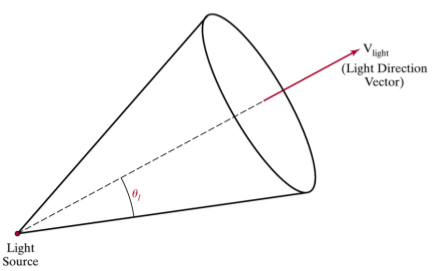
\includegraphics[width=0.48\textwidth]{Figures/Hol}
			\end{center}
	\end{figure}	
	
\end{frame}


%%%%%%%%%%%%%%%%%%%%%%%%%%%%%%%%%%%%%%%%%%%%%%%%%%%%%%%%%%%%%%%%%%%%%%%%%%%%%%%%%%%%%%%%%%

\begin{frame}
\frametitle{Fontes de Luz}

	\begin{block}{Efeito de Holofote}
		\begin{itemize}
			\item Podemos utilizar dois vetores para direcionar a luz.
			\begin{itemize}
				\item Um vetor $\textbf{V}_{light}$ para direcionar a luz.
				\item Um vetor $\textbf{V}_{obj}$ para direcionar a luz a um objeto.
			\end{itemize}
			\item Considerando que $cos \alpha = \textbf{V}_{light} \cdot \textbf{V}_{obj}$ e limitando $0^\circ \leq \theta_l \leq 90^\circ$, então o objeto está dentro da região de luz se $cos \alpha \geq cos \theta_l$				 
		\end{itemize}
	\end{block}

	\begin{figure}[!h]
			\begin{center}
			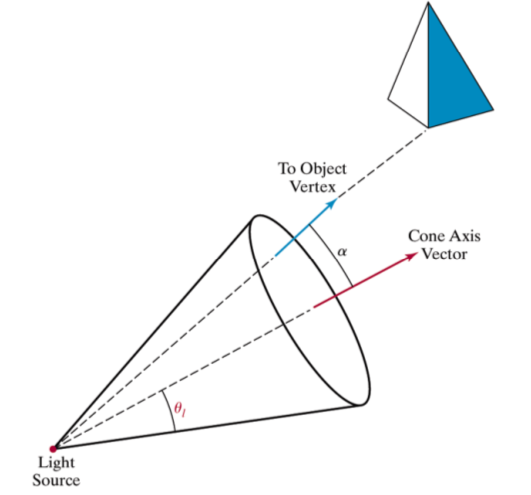
\includegraphics[width=0.35\textwidth]{Figures/OloVec}
			\end{center}
	\end{figure}	
	
\end{frame}

%%%%%%%%%%%%%%%%%%%%%%%%%%%%%%%%%%%%%%%%%%%%%%%%%%%%%%%%%%%%%%%%%%%%%%%%%%%%%%%%%%%%%%%%%%
\begin{frame}
\frametitle{Fontes de Luz}

	\begin{block}{Atenuação Angular de Intensidade}
		\begin{itemize}
			\item Para uma fonte de luz direcional a atenuação ocorre \textbf{angularmente} e \textbf{radialmente} a partir da posição da fonte.
			\begin{itemize}
				\item Assim é possível simular cones de luz que são mais intensos ao longo do cone.
			\end{itemize}								 
		\end{itemize}
	\end{block}

	\begin{figure}[!h]
			\begin{center}
			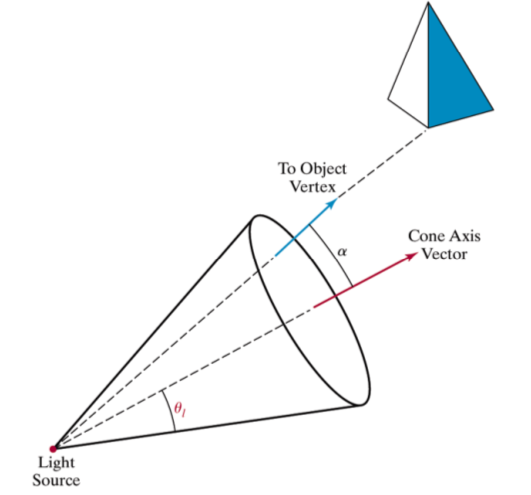
\includegraphics[width=0.35\textwidth]{Figures/OloVec}
			\end{center}
	\end{figure}	
	
\end{frame}

%%%%%%%%%%%%%%%%%%%%%%%%%%%%%%%%%%%%%%%%%%%%%%%%%%%%%%%%%%%%%%%%%%%%%%%%%%%%%%%%%%%%%%%%%%
\begin{frame}
\frametitle{Fontes de Luz}

	\begin{block}{Atenuação Angular de Intensidade}
		\begin{itemize}
			\item Para uma fonte de luz direcional a atenuação ocorre \textbf{angularmente} e \textbf{radialmente} a partir da posição da fonte.
			\begin{itemize}
				\item Assim é possível simular cones de luz que são mais intensos ao longo do cone.
			\end{itemize}	
			\item Uma função de atenuação é:
				\begin{equation*}
					f_{angatten}(\phi) = cos^{a_t} \phi, 0^\circ \leq \phi \leq \theta
				\end{equation*}	
			\item Onde $a_t$ é o expoente de atenuação e $\phi$ é o ângulo medido a partir do eixo do cone.
			\begin{itemize}
				\item Ao longo do eixo temos $\phi = 0^\circ$ e $f_{angatten}(\phi) = 1$.
				\item Quanto maior o valor de $a_t$ menor o valor de $f_{angatten}$ com $\phi > 0^\circ$
\end{itemize}													 
		\end{itemize}
	\end{block}
	
\end{frame}

%%%%%%%%%%%%%%%%%%%%%%%%%%%%%%%%%%%%%%%%%%%%%%%%%%%%%%%%%%%%%%%%%%%%%%%%%%%%%%%%%%%%%%%%%%
\begin{frame}
\frametitle{Fontes de Luz}

	\begin{block}{Atenuação Angular de Intensidade}
		\begin{itemize}
			\item Considerando os vetores $\textbf{V}_{light}$ e $\textbf{V}_{obj}$ e assumindo $0^\circ \leq \theta_l \leq 90^\circ$ a equação geral da atenuação pode ser definida como:							$fa = \left\{
					\begin{array}{l l}
   						 1 & \quad \text{se a fonte de luz não é direcional}\\
   						 0 & \quad \text{Se } \textbf{V}_{light} \cdot \textbf{V}_{obj} = cos \alpha < cos \theta_l\\
   						  & \quad \text{Objeto está fora}\\
    						(\textbf{V}_{light} \cdot \textbf{V}_{obj})^{al} & \quad \text{caso contrário}
  					\end{array} \right.$
		\end{itemize}
	\end{block}
	
\end{frame}

%%%%%%%%%%%%%%%%%%%%%%%%%%%%%%%%%%%%%%%%%%%%%%%%%%%%%%%%%%%%%%%%%%%%%%%%%%%%%%%%%%%%%%%%%%
\begin{frame}
\frametitle{Fontes de Luz}

	\begin{block}{Fontes de Luz Estendidas e o Modelo de Warn}
		\begin{itemize}
			\item Para se incluir uma fonte de luz grande em uma posição próxima aos objetos da cenas, podemos aproximar esse efeito como uma superfície que emite luz.
			\item Este efeito pode ser modelado utilizando uma grade de fontes direcionais.
		\end{itemize}
	\end{block}
	
	\begin{figure}[!h]
			\begin{center}
			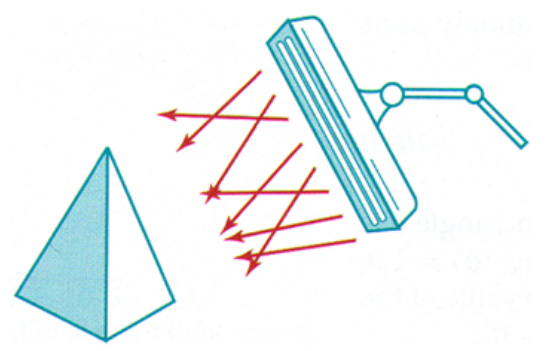
\includegraphics[width=0.35\textwidth]{Figures/FonLuzGra}
			\end{center}
	\end{figure}	
	
\end{frame}


%%%%%%%%%%%%%%%%%%%%%%%%%%%%%%%%%%%%%%%%%%%%%%%%%%%%%%%%%%%%%%%%%%%%%%%%%%%%%%%%%%%%%%%%%%
\section{Fontes de Luz em Superfícies}
\begin{frame}
\frametitle{Efeito de Luz em Superfícies}

	\begin{block}{Efeito de Luz em Superfícies}
		\begin{itemize}
			\item Um modelo de iluminação computa os \textbf{efeitos de luz} levando em consideração 	várias \textbf{propriedades óticas}.
			\item Quando uma superfícies é \textbf{Opaca}, parte da luz é refletida e parte é absorvida.
			\begin{itemize}
				\item A quantidade de luz refletida depende do tipo de material da superfície.
			\end{itemize}
			\item Em superfícies transparentes, alguma luz é transmitida através da mesma.
		\end{itemize}
	\end{block}
	
\end{frame}

%%%%%%%%%%%%%%%%%%%%%%%%%%%%%%%%%%%%%%%%%%%%%%%%%%%%%%%%%%%%%%%%%%%%%%%%%%%%%%%%%%%%%%%%%%
\begin{frame}
\frametitle{Efeito de Luz em Superfícies}

	\begin{block}{Reflexão Difusa}
		\begin{itemize}
			\item Superfícies irregulares tendem a refletir luz em todas as direções, tendo a impressão de ser igualmente brilhante quando vista de qualquer ponto.
			\item A cor do objeto é a cor da reflexão difusa com uma iluminação branca.
					\begin{itemize}
						\item Objetos azuis refletem a componente azul na cor branca.
						\item Um objeto azul sobre a luz vermelha ficará preto pois o vermelho reflete  absorve todo o azul.
					\end{itemize}							
		
		\end{itemize}
	\end{block}
	
	\begin{figure}[!h]
			\begin{center}
			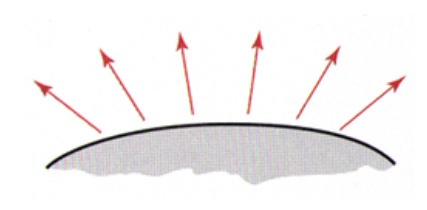
\includegraphics[width=0.35\textwidth]{Figures/RefDif}
			\end{center}
		\end{figure}	
	
\end{frame}

%%%%%%%%%%%%%%%%%%%%%%%%%%%%%%%%%%%%%%%%%%%%%%%%%%%%%%%%%%%%%%%%%%%%%%%%%%%%%%%%%%%%%%%%%%
\begin{frame}
\frametitle{Efeito de Luz em Superfícies}

	\begin{block}{Reflexão Especular}
		\begin{itemize}
			\item Alguma parte da luz é concentrada em uma região mais brilhante.
			\item O realce é maior em superfícies brilhantes.
		\end{itemize}
	\end{block}
	
	\begin{figure}[!h]
			\begin{center}
			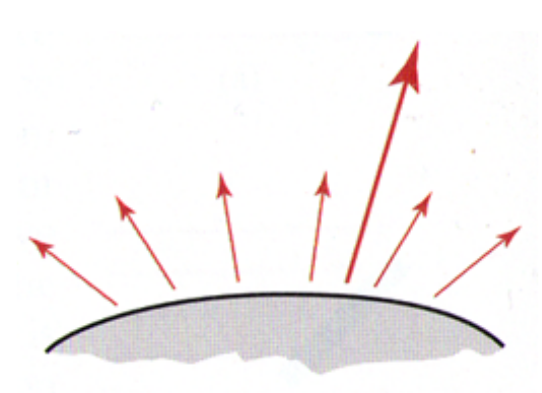
\includegraphics[width=0.35\textwidth]{Figures/LuzEsp}
			\end{center}
		\end{figure}	
	
\end{frame}

%%%%%%%%%%%%%%%%%%%%%%%%%%%%%%%%%%%%%%%%%%%%%%%%%%%%%%%%%%%%%%%%%%%%%%%%%%%%%%%%%%%%%%%%%%
\begin{frame}
\frametitle{Efeito de Luz em Superfícies}

	\begin{block}{Luz de Fundo ou Ambiente}
		\begin{itemize}
			\item Efeito da luz produzida pela luz refletida no ambiente de várias superfícies.
			\begin{itemize}
				\item A luz total refletida de uma superfície é a soma das contribuições da luz refletida pelas outras superfícies.
			\end{itemize}
		\end{itemize}
	\end{block}
	
	\begin{figure}[!h]
			\begin{center}
			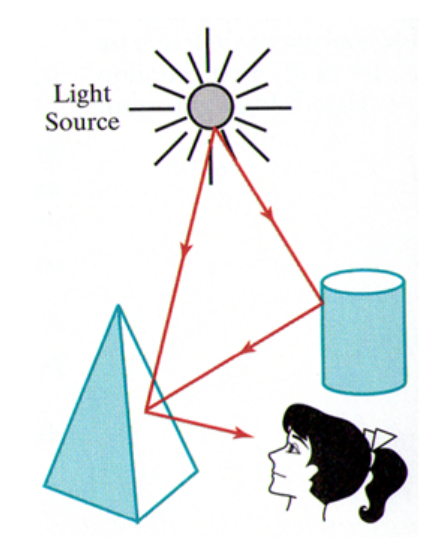
\includegraphics[width=0.35\textwidth]{Figures/LuzAmb}
			\end{center}
		\end{figure}	
	
\end{frame}

%%%%%%%%%%%%%%%%%%%%%%%%%%%%%%%%%%%%%%%%%%%%%%%%%%%%%%%%%%%%%%%%%%%%%%%%%%%%%%%%%%%%%%%%%%
\section{Modelos Básicos de Iluminação}
\begin{frame}
\frametitle{Modelos Básicos de Iluminação}

	\begin{block}{Modelos Básicos de Iluminação}
		\begin{itemize}
			\item \textbf{Modelos Precisos} de iluminação computam toda a iteração entre a radiação de luz e o material do objeto.
			\item Contudo esta iteração é computacionalmente muito \textbf{cara}.
			\item Assim algumas aproximações para a iluminação ambiente são definidas.
		\end{itemize}
	\end{block}
	
\end{frame}

%%%%%%%%%%%%%%%%%%%%%%%%%%%%%%%%%%%%%%%%%%%%%%%%%%%%%%%%%%%%%%%%%%%%%%%%%%%%%%%%%%%%%%%%%%
\begin{frame}
\frametitle{Modelos Básicos de Iluminação}

	\begin{block}{Luz Ambiente}
		\begin{itemize}
			\item A luz de fundo pode ser incorporada definindo um \textbf{brilho geral} para a cena.
			\begin{itemize}
				\item Produz uma luz ambiente que uniforme para todos os objetos, gerando uma aproximação da reflexão difusa de todas as superfícies da cena.
			\end{itemize}
			\item A quantidade de luz refletida depende do material (propriedades óticas) das superfícies.
			\item O nível de luz ambiente em uma cena é definido por um parâmetro de intensidade $I_a$.
		\end{itemize}
	\end{block}
	
\end{frame}

%%%%%%%%%%%%%%%%%%%%%%%%%%%%%%%%%%%%%%%%%%%%%%%%%%%%%%%%%%%%%%%%%%%%%%%%%%%%%%%%%%%%%%%%%%
\begin{frame}
\frametitle{Modelos Básicos de Iluminação}

	\begin{block}{Reflexão Difusa}
		\begin{itemize}
			\item A reflexão difusa pode ser modelada assumindo que a luz incidente é \textbf{espalhada com igual intensidade} em todas as direções independente da direção de visão.
			\begin{itemize}
				\item Estas superfícies são denominadas \textbf{refletores difusos ideais} (refletores Lambertinianos).
			\end{itemize}
			\item Assumindo que toda superfície é um refletor difuso ideal, um parâmetro $k_d$(\textbf{coeficiente de reflexão difusa}) pode ser utilizado para determinar a fração de luz incidente que irá se espalhar com reflexão.
								 
		\end{itemize}
	\end{block}
	
\end{frame}

%%%%%%%%%%%%%%%%%%%%%%%%%%%%%%%%%%%%%%%%%%%%%%%%%%%%%%%%%%%%%%%%%%%%%%%%%%%%%%%%%%%%%%%%%%
\begin{frame}
\frametitle{Modelos Básicos de Iluminação}

	\begin{block}{Reflexão Difusa}
		\begin{itemize}
			\item Para fontes de luz monocromáticas, $0 \leq k_d \leq 1.0$
			\begin{itemize}
				\item Superfícies brilhantes possuem $k_d$ altos.
				\item Superfícies que absorvem luz possuem $k_d$ próximos de 0.
			\end{itemize}						 
		\end{itemize}
	\end{block}
	
\end{frame}

%%%%%%%%%%%%%%%%%%%%%%%%%%%%%%%%%%%%%%%%%%%%%%%%%%%%%%%%%%%%%%%%%%%%%%%%%%%%%%%%%%%%%%%%%%
\begin{frame}
\frametitle{Modelos Básicos de Iluminação}

	\begin{block}{Reflexão Difusa}
		\begin{itemize}
			\item Para efeitos de luz de fundo, as superfícies são completamente iluminadas pelas luz ambiente $I_a$. A contribuição da reflexão difusa é:
				\begin{equation*}
					I_{reflecdiff} = k_d \cdot I_a
				\end{equation*}						 
		\end{itemize}
	\end{block}
	
\end{frame}



%----------------------------------------------------------------------------------------
\end{document} 